How does analog sorting compare to other sorting algorithms for example quick, merge etc in terms of complexity?

\subsection{Functionality validation of analog sorting}
\begin{figure}
\centering
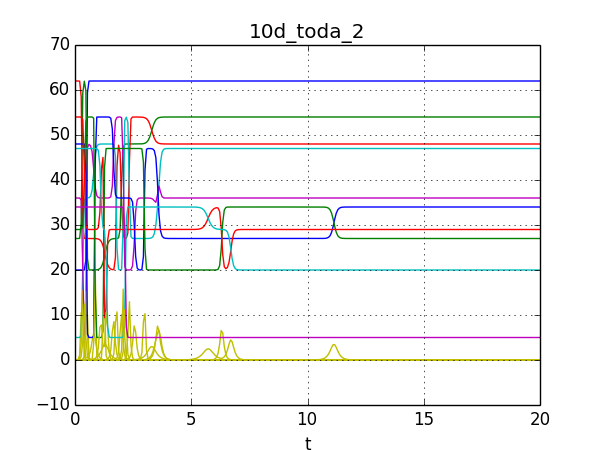
\includegraphics{../pyscripts/Graphs/10d_toda_2.png}
\caption{A sample black and white graphic.}
\end{figure}

\subsection{Time cost of the discrete QR algorithm}
Time cost of overall QR loop:
	how many iterations of qr til convergence?
	% time to convergence of qr w.r.t.. problem size
	Since we know the ODE is analogous to QR algorithm, they should take the same amount of time.
Time cost of QR step:
	Numerical Recipes 3rd Edition p585 says the QR algorithm takes O(N) time for symmetric tridiagonal matrices.

\subsection{Time cost of analog sorting}
% \begin{figure}
% \centering
% \includegraphics{fly}
% \caption{A sample black and white graphic.}
% \end{figure}

\subsection{Hardware cost of analog sorting}
Time cost of analog sorting
	In terms of time, the sorter takes at least O(N) time because of the time it takes just for signals to propagate across the circuit.
	Another issue is the time it takes for the ODE to settle to its final value.

Hardware cost of analog sorting
The analog sorter takes up O(N) amount of circuit components to sort N elements.







% \begin{figure}
% \centering
% \includegraphics[height=1in, width=1in]{fly}
% \caption{A sample black and white graphic
% that has been resized with the \texttt{includegraphics} command.}
% \end{figure}


% \begin{figure*}
% \centering
% \includegraphics{flies}
% \caption{A sample black and white graphic
% that needs to span two columns of text.}
% \end{figure*}


% \begin{figure}
% \centering
% \includegraphics[height=1in, width=1in]{rosette}
% \caption{A sample black and white graphic that has
% been resized with the \texttt{includegraphics} command.}
% \vskip -6pt
% \end{figure}

